\vspace{-3mm}
\section{}
\vspace{-4mm}
%%------------------------------------------------------------------------------------------
%                                   section intro 2 column
%%------------------------------------------------------------------------------------------
\begin{multicols}{2}
    \begin{minipage}{\columnwidth}
    \vspace{2mm}
    \centering%
    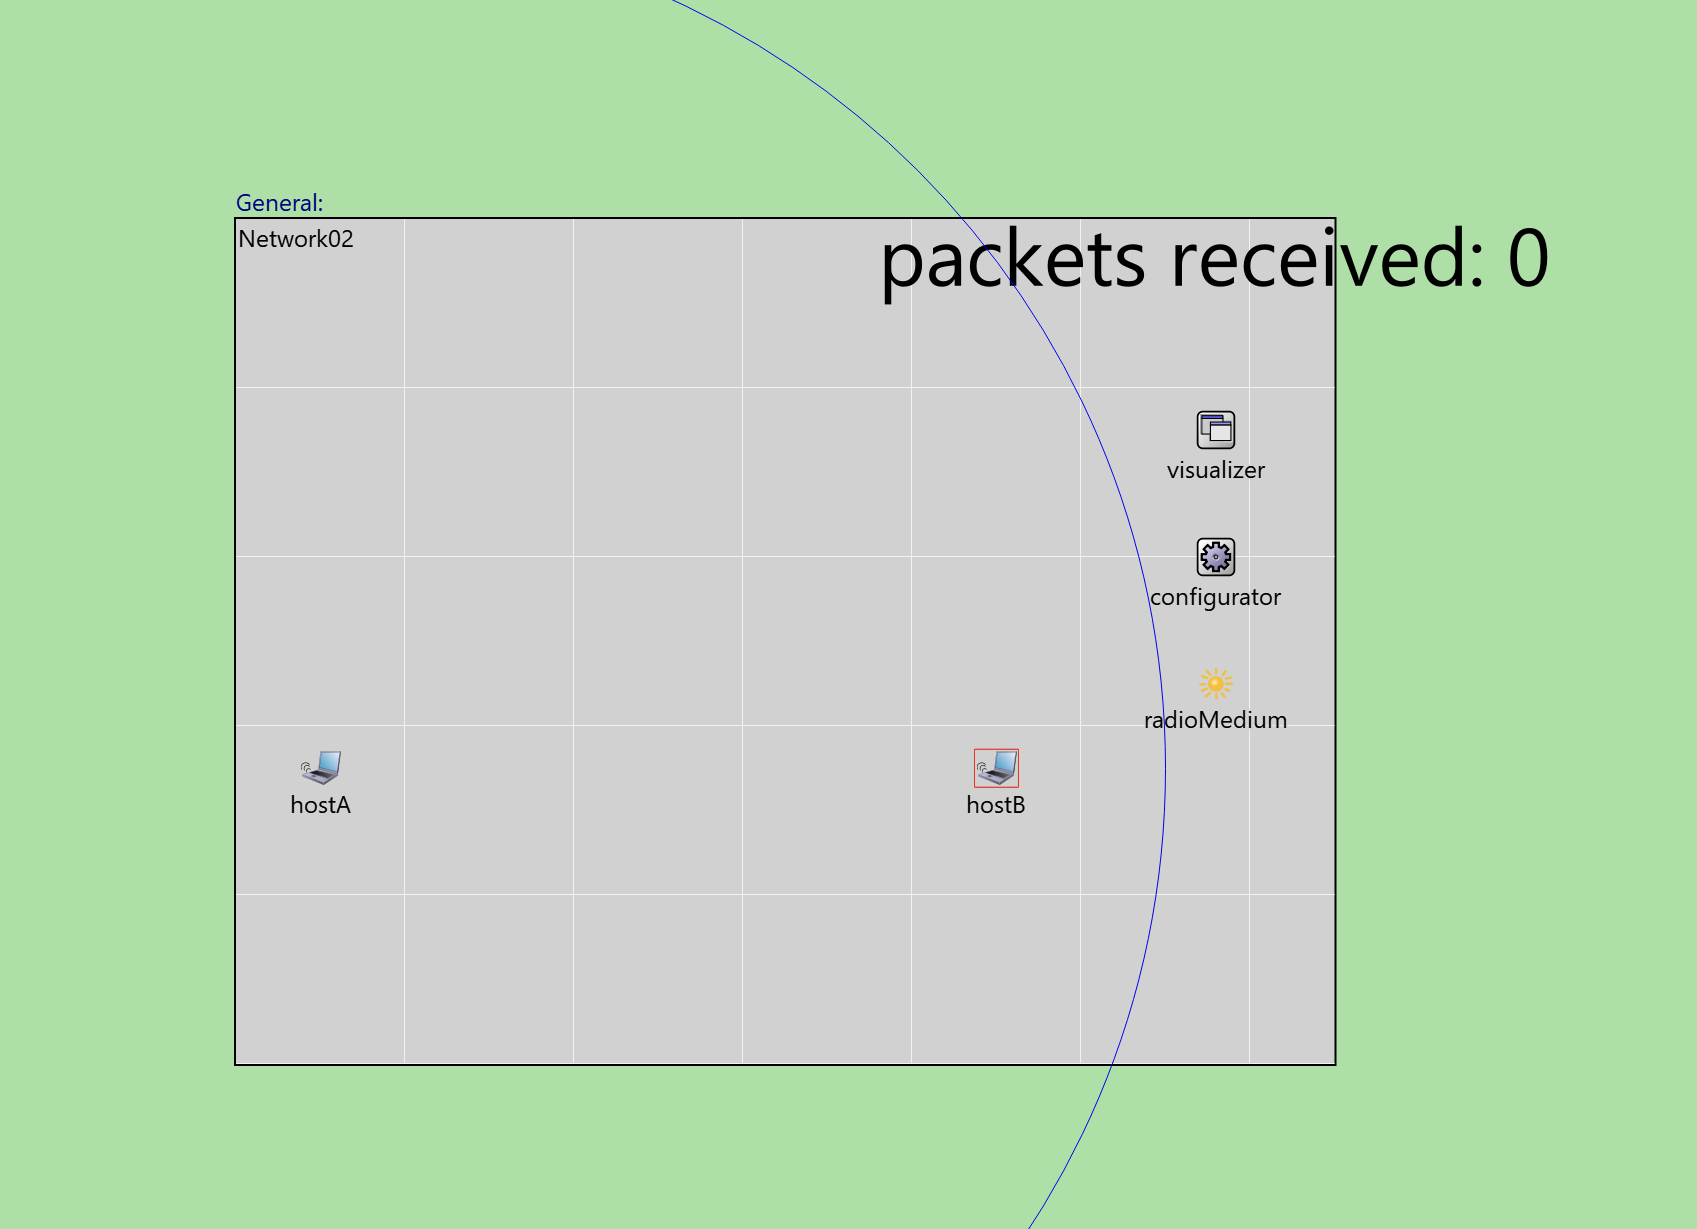
\includegraphics[width=.9\textwidth]{image/week12/2-1.png}
    \vspace{-2mm}
    \captionof{figure}{\small Hidden Node Problem Diagram}    \vspace{-4mm}
    \end{minipage}
    
    \columnbreak
    
    Experiment 2,3,4 에서는 INET framework 에서 무선 시뮬리에션을 구축해 본다.
    
    Experiment 2 에서는 무선으로 통신하는 2 HOST의 simulation 실험으로,  한 HOST가 다른 HOST에게 UDP 데이터 스트림을 무선으로 보내는 네트워크를  구성한다.
    HOST A가 1000 byte 크기의 UDP packet을 생성하여 HOST B 에게 평균 10ms의exponential distribution을 가지는 무작위 간격으로 전송한다.
    이때 2개의 host의 간격은 400m로, ini 에서 설정해준 network의 유효 통신범위radio.transmitter.communicationRange 의 500m 이내이므로 직접 통신이 가능한 기본적인 네트워크에서 simulation을 진행한다.
    \vspace{-4mm}
\end{multicols}
\vspace{-4mm}
%%%%%%%%%%%%%%%%%%%%%%%%%%%%%%%%%%%%%%%%%%%%%%%%%%%%%%%%%%%%%%%%%%%%%%%%%%%%%%%%%%%%%%%%%%%%
%%------------------------------------------------------------------------------------------
%                                   Cose Reference
%%------------------------------------------------------------------------------------------
\vspace{-4mm}
\subsection*{CODE}
\vspace{-3mm}
lecture 에서 blank를 채운 코드이외에 lecrure에서 주어진 실행 code들은 보고서 마지막 appendix에 첨부했다.
\vspace{-3mm}
    \subsubsection*{Network02.ompnetpp.ini}
        \vspace{-2mm}
        \begin{listing}[h!]
        \inputminted[framerule = 1pt,framesep = 2mm , frame = lines, fontsize=\scriptsize]{c}{./code/week12/Experiment_02/ini.cpp}
        \vspace{-3mm}
        \caption{\footnotesize Network02.ned}
        \vspace{-3mm}
        \end{listing}
        \vspace{-6mm}
\clearpage
%%%%%%%%%%%%%%%%%%%%%%%%%%%%%%%%%%%%%%%%%%%%%%%%%%%%%%%%%%%%%%%%%%%%%%%%%%%%%%%%%%%%%%%%%%%%
%%------------------------------------------------------------------------------------------
%           simulation results -> you tube 링크 + 스크린샷 2장 + 내용에 대한 설명
%%------------------------------------------------------------------------------------------
\subsection*{SIMULATION RESULTS}
    \vspace{-1mm}
    Host A 에서 Host B로 UDP packet을 전송하는 동작을 네트워크 외부, Host A 내부, Host B 내부 동작의 화면녹화 영상을 업로드하였다.
    simulation 전체의 영상은 아래 링크를 클릭하여 확인할 수 있다.     
    \vspace{-10mm}
        \begin{center}
            \item \href{https://youtu.be/N8wHft9a8jM}
        	{Youtube link of Week12 Experiment 02 Simulation Results Screenshot Video}
        \end{center}
    \vspace{-6mm}
    % 사진 1 2개는 넣어 주자
        \begin{figure}[h!]
        \centering
        \subfloat{
            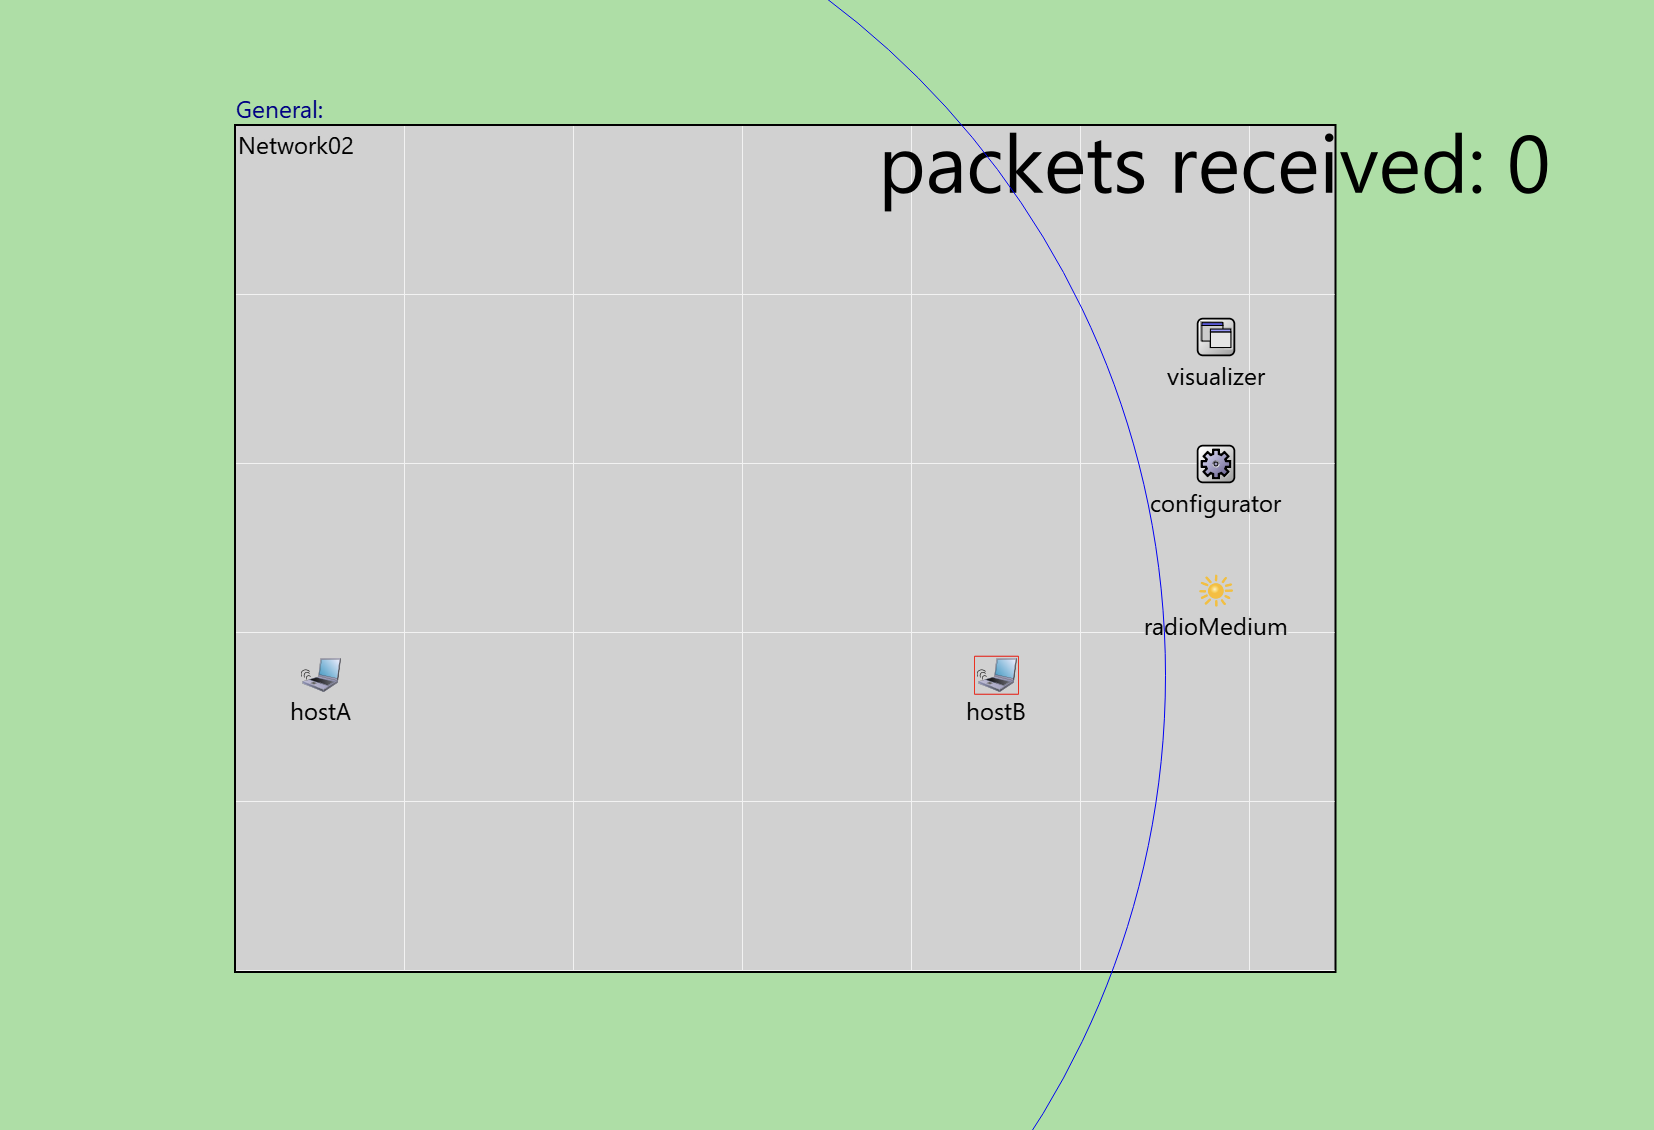
\includegraphics[width=0.46\textwidth]{image/week12/2-2-1.png}
        }\hspace{3mm}
        \subfloat{
            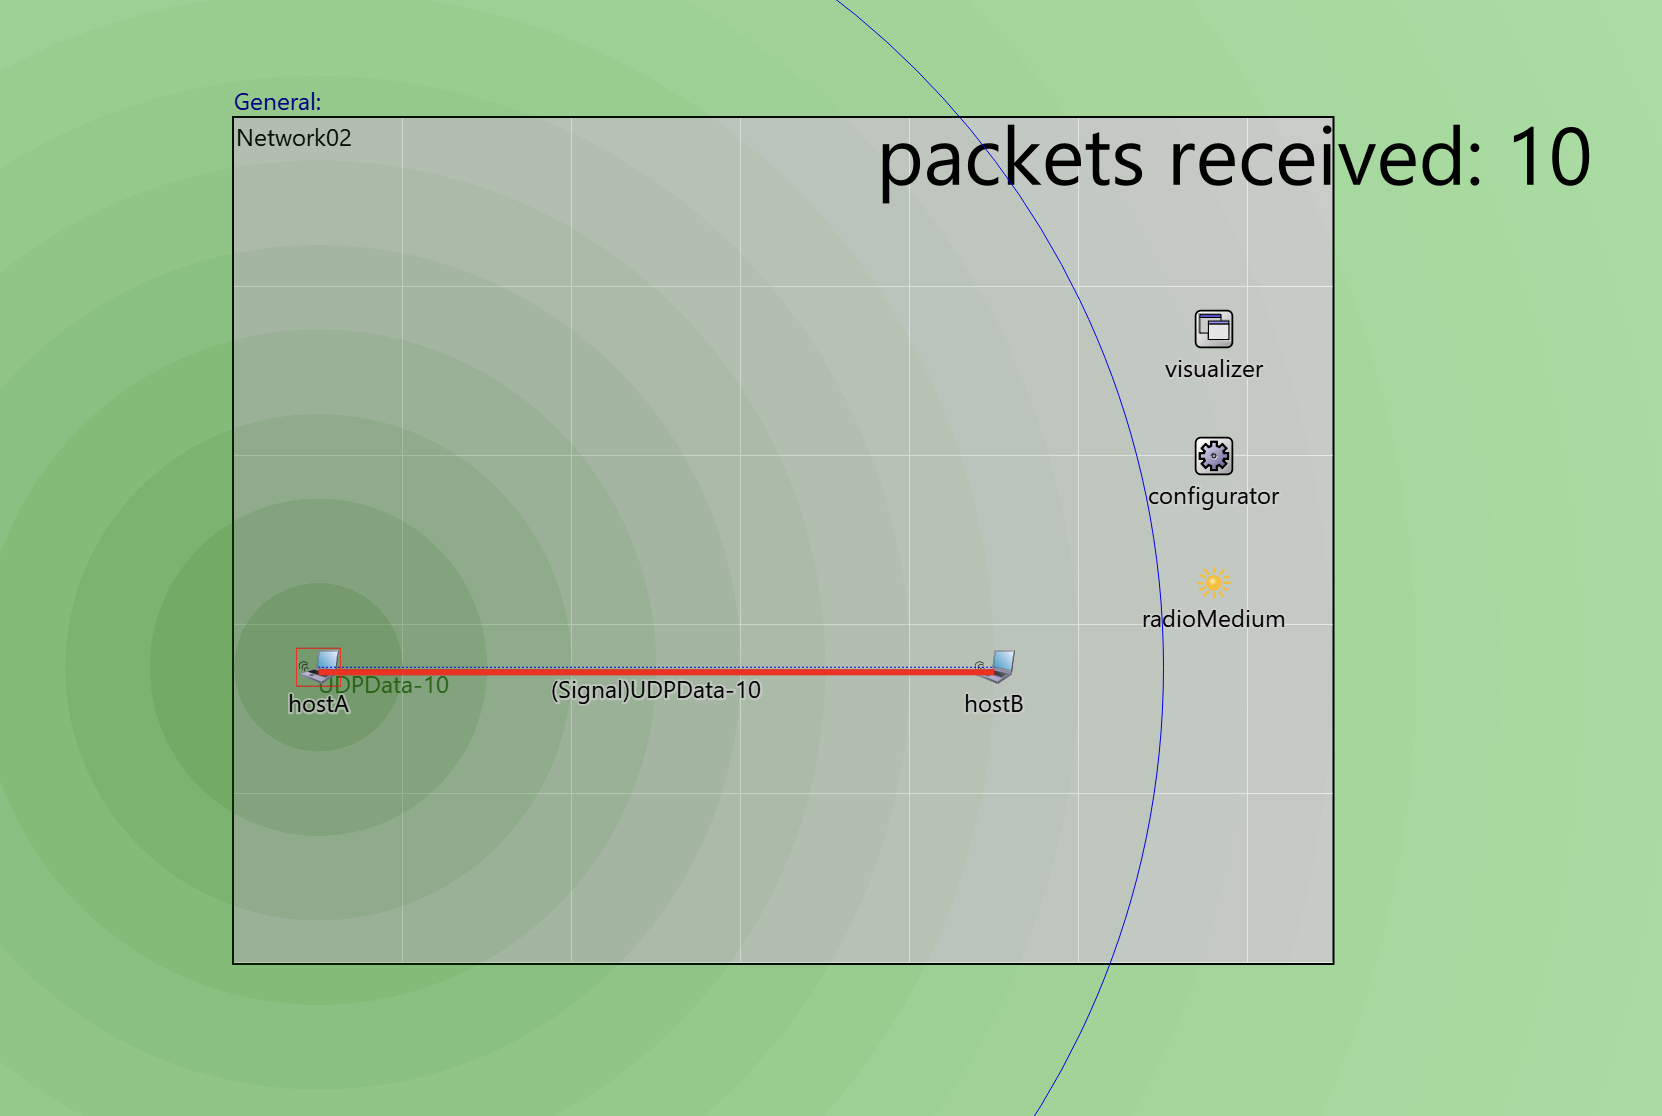
\includegraphics[width=0.46\textwidth]{image/week12/2-2-2.png}
        }
        \caption{Experiment 02 Simulation Results Screenshot}
        \vspace{-2mm}
        \end{figure}
    
    simulation 의 flow는 다음과 같다. 
\vspace{-3mm}
    \subsubsection*{Transfer Model }
    \vspace{-2mm}
    Host A 가 Host B에게 전송하는 10ms 의 exponential 한 분포를 따르는 무작위 간격으로 1000 바이트 크기의 UDP 트래픽을 생성해 전송한다.  그리고 ini 에 추가해준 visulaize함수로 Host B 가 받은 패킷수를 표기해 주었다. 
\vspace{-1mm}
    \subsubsection*{Physical Layer Modelling }
    \vspace{-2mm}
    ini 에서 가능한 무선 통신 연결거리를 500m, 1Mbps의 속도로 데이터가 전송이되고, ned 에서 Host A 와 Host B의 간격을 450m 로 설정해주어 직접 통신이 가능하도록 설정해 주었다. 
    \subsubsection*{Simulation Scenario}
    Host A 에서 임의의 간격으로 UDP pacjet을 생성해주고, 생성된 packet은 IPv4 를 통해서네트워크 later로 이동한다. 이때 네트워크 layer에서 packet은 전송 대기열이 진행하는 simulation처럼 없으면 바로 전송이 이뤄진다. 이후 Host A 에서 Host B로 바로 모든 packet이 전송된다.
    
\clearpage